\documentclass[12pt]{article}

\usepackage[utf8]{inputenc}
\usepackage[T1]{fontenc}
\usepackage[brazil]{babel}
\usepackage{graphicx}
\usepackage{cancel}

\usepackage{geometry}
\geometry{margin=2.5cm}
\usepackage{setspace}
\onehalfspacing

\usepackage{amsmath, amssymb, amsthm}
\usepackage{mathtools}

\numberwithin{equation}{section}

\theoremstyle{plain}
\newtheorem{theorem}{Teorema}[section]
\newtheorem{proposition}[theorem]{Proposição}
\newtheorem{lemma}[theorem]{Lema}
\newtheorem{corollary}[theorem]{Corolário}

\theoremstyle{definition}
\newtheorem{definition}[theorem]{Definição}
\newtheorem{example}[theorem]{Exemplo}
\newtheorem{exercise}{Exercício}

\theoremstyle{remark}
\newtheorem*{remark}{Observação}

\usepackage{hyperref}
\usepackage{csquotes}

\usepackage[
    backend=biber,
    style=authoryear,
    maxcitenames=2
]{biblatex}

\addbibresource{/mnt/c/Users/nicho/Documents/nicholasvoltani.github.io/bibliography.bib}

\newcommand{\R}{\mathbb{R}}
\newcommand{\pref}{\succeq}
\newcommand{\strictpref}{\succ}
\newcommand{\indiff}{\sim}

% ------------------------------------------------
% Title (fill manually)
% ------------------------------------------------
\title{Lista 2 -- Teoria Microeconômica}
\author{Professor: Fábio Waltenberg \\Monitor: Nicholas Funari Voltani}
\date{}

\begin{document}
\maketitle

\hypertarget{conceitos-introdutuxf3rios}{%
\section{Conceitos introdutórios}\label{conceitos-introdutuxf3rios}}



\hypertarget{exercuxedcios}{%
\section{Exercícios}\label{exercuxedcios}}

\begin{exercise}
    Um consumidor consome um bem de consumo \(x\) e
    usufrui de uma quantidade de horas de lazer \(h\). O preço do bem de
    consumo é \(p\), e o consumidor pode trabalhar a uma taxa salarial de
    \(s \in \mathbb{R}^+\) (salário \emph{positivo}!). Qual é o conjunto
    orçamentário walrasiano do consumidor, em notação matemática? Note que
    \(0 \leq h \leq 24\), e que o consumidor divide seu tempo entre lazer (um bem que usufrui) e trabalho assalariado (um ``mal'').
\end{exercise}

\begin{exercise}
    Uma função de utilidade de Cobb-Douglas de uma
    dada cesta de \(n\) bens \(\vec{x}=(x_{1},\dots,x_{n})\) é definida como
    \[
    U(x_{1},\dots,x_{n}) = \prod\limits_{i=1}^{n} x_{i}^{\alpha_{i}} = x_{1}^{\alpha_{1}}x_{2}^{\alpha_{2}}\dots x_{n}^{\alpha_{n}}
    \] em que \(\sum\limits_{i=1}^{n} \alpha_{i} = 1\). Supondo que o vetor
    de preços é \(\vec{p}=(p_{1},\dots,p_{n}) \in \mathbb{R}^{n}_{+}\) e que
    a restrição orçamentária seja \[
    \left\{  \vec{x} \in \mathbb{R}^n : \vec{x} \cdot \vec{p} = \sum \limits_{i=1}^{n} x_{i}p_{i} \leq w  \right\}
    \]Mostre, através da maximização da utilidade via multiplicadores lagrangianos, que a
    demanda walrasiana, para cada bem \(i = 1, \dots, n\), é da forma \[
    x^*_{i}(p,w) = \alpha_{i} \frac{w}{p_{i}}
    \]
    
    Calcule também a elasticidade-renda \(\epsilon_{lw}(p,w)\) dessa
    demanda.

    \textbf{Dica}: Note que as condições de multiplicadores lagrangianos dão
    a seguinte identidade, para cada \(i,j = 1, \dots, n\): 
    \[
    \frac{\alpha_{i}}{p_{i} x^*_{i}} = \frac{\alpha_{j}}{p_{j} x^*_{j}}
    \] 
    Através dela, verifique que se pode concluir que a demanda ótima de
    Cobb-Douglas é tal que \[
    \alpha_{i} = \frac{p_{i}x_{i}}{w}
    \] Ou seja, os coeficientes \(\alpha_{i} \in (0, 1]\) do bem \(i\) dão o percentual
    da renda (\(=w\)) que é despendida no bem \(i\) (\(=p_{i}x_{i}\)).
    
\end{exercise}

\begin{exercise}
    Uma função de utilidade quase-linear em
    \(\mathbb{R}^{2}\) tem a forma \[
    U(x_{1},x_{2}) = x_{1} + v(x_{2})
    \] onde \(v(x)\) é alguma função. Seja
    \(\vec{p}=(p_{1},p_{2}) \in \mathbb{R}^{2}_{+}\) o vetor de preços, e
    uma restrição orçamentária dada por \(w \in \mathbb{R}\).
    
    Calcule a demanda walrasiana \(\vec{x}^*\) para
    \(v(x_{2}) = \sqrt{ x_{2} }\) e para \(v(x_{2}) = \ln x_{2}\). Calcule também a elasticidade-renda \(\epsilon_{lw}(p,w)\) dessa demanda.

    \begin{remark}
        Note que essas demandas walrasianas não determinam \(x_{1}\)! Isso quer
        dizer que, dados \(\vec{p}\) e \(w\), o conjunto de cestas \[
        \{ m \in \mathbb{R}: (m,x_{2}^*) \}
        \] dado o \(x_{2}^*\) ótimo, são todas cestas ótimas.   
    \end{remark}

\end{exercise}

\begin{exercise}
    Uma função de utilidade CES\footnote{\textit{Constant Elasticity of Substitution}.} é da forma \[
    U(x_{1},x_{2}) = (\alpha_{1} x_{1}^\rho + \alpha_{2}x_{2}^\rho)^{1/\rho}
    \] para dado \(\rho \in (-\infty, 1]\). Dado vetor de preços
    \(\vec{p} = (p_{1},p_{2}) \in \mathbb{R}^{2}\) e restrição orçamentária
    \(w\), obtenha a demanda walrasiana \(\vec{x}^*\). Calcule também a elasticidade-renda \(\epsilon_{lw}(p,w)\) dessa demanda.

    \textbf{Dica}: Conforme exercício 3 da lista 1, a demanda ótima de \(U(\vec{x})\) é a mesma que a de\footnote{$\coloneqq$ é um símbolo que indica uma definição de uma nova variável.} \(\tilde{U}(\vec{x}) \coloneqq \rho \, U(\vec{x})^{\rho} = \rho \, (\alpha_{1} x_{1}^\rho + \alpha_{2}x_{2}^\rho)\),
    o que facilita os cálculos.

\end{exercise}

\begin{exercise}
    Dada a função de utilidade CES (vide acima) --- com pesos $\alpha_i$ iguais (ninguém é de ferro) ---, demonstre que ela tende às funções de utilidade 
    \begin{enumerate}
        \item linear quando \(\rho \to 1\)
        \item Cobb-Douglas quando \(\rho \to 0\) (supondo que \(\alpha_{1} + \alpha_{2} = 1\)). \textbf{Dica}: Caso não tenha resolvido o exercício acima, pode ser útil fazer o limite para \(\tilde{U}(\vec{x}) = \ln U(\vec{x}) = \frac{1}{\rho} \ln(\alpha_{1} x_{1}^\rho + \alpha_{2}x_{2}^\rho)\). Além disso, lembre-se que, embora \(\frac{ \partial x^\rho }{ \partial x } = \rho x^{\rho - 1}\), temos que\footnote{Rigorosamente, só podemos fazer $z = \exp(\ln z)$ se $z > 0$. Esta condição é satisfeita, pois estamos sempre falando de cestas de bens que tenham ao menos "um pouco de cada bem". Sim, estamos fugindo de Kuhn-Tucker como o diabo foge da cruz!} \(\frac{ \partial x^\rho }{ \partial \rho } = \frac{ \partial }{ \partial \rho } \exp(\ln x^\rho) = \ln(x) x^\rho\) --- uma derivada que \textbf{não é em relação a \(x\)}!)
    \item Leontief quando \(\rho \to -\infty\)
    \end{enumerate}

    \textbf{Recomendação}: Uma boa visualização da função CES pode ser
    encontrada em
    \href{https://www.econgraphs.org/textbooks/intermediate_micro/scarcity_and_choice/preferences_and_utility/ces.html}{CES
    Utility Function - EconGraphs}.

\end{exercise}


\begin{exercise}
    Mostre que as elasticidades de substituição
    \(\xi_{12}\) da função de utilidade CES são 
    
    \begin{enumerate}
        \item \(\xi_{12} \to -\infty\) quando \(\rho \to 1\) (utilidade linear) 
        \item \(\xi_{12} \to -1\) quando \(\rho \to 0\) (utilidade Cobb-Douglas) 
        \item \(\xi_{12} \to 0\) quando \(\rho \to -\infty\) (utilidade de Leontief)
    \end{enumerate}
\end{exercise}


\begin{exercise}
    Mostre que, se uma demanda walrasiana
    \(x(p,w) \in \mathbb{R}^L\) (\(x\) é um vetor de \(L\) elementos) é
    homogênea de grau \(1\) em relação a \(w\) --- isto é,
    \(x(p, \alpha w) = \alpha x(p,w)\) ---, e satisfaz a lei de Walras,
    então \[
    \epsilon_{lw}(p, w) = 1 \,\, (l = 1, 2, \dots, L)
    \] O que isso quer dizer sobre
    \(\frac{ \partial x_{l}(p,w) }{ \partial w}\) e, portanto, sobre a
    respectiva curva de Engel desta demanda?

\end{exercise}

\vfill 

\pagebreak

\section{Resoluções}

\setcounter{exercise}{0}

\begin{exercise}
    Dados os bens \(x\) e \(h\), onde \(x\) possui preço \(p\) e o tempo de trabalho possui salário \(s\), temos que a restrição orçamentária é de que 
    \[
\underbrace{ p\cdot x }_{ \text{Consumo de bens} } \leq \underbrace{ (24-h)\cdot s }_{ \text{Salário} } 
\] 
o que é equivalente a 
\[ \underbrace{ p \cdot x + s \cdot h }_{ \text{Custos (+ de oportunidade)} } \leq \underbrace{ 24 \cdot s }_{ \text{Salário máximo} }
\]

\begin{figure}[h]
    \centering
    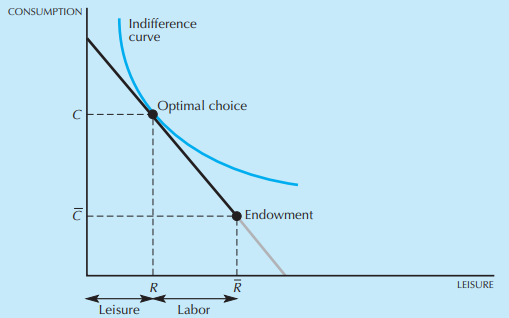
\includegraphics{images/Pasted image 20250424141222.png}
    \caption{(Varian, 2014, p. 175).}
\end{figure}
\end{exercise}

\begin{exercise}
    A Função de Cobb-Douglas geral tem a forma \[
U(x_{1},\dots,x_{L}) = \prod \limits_{k=1}^{L} x_{k}^{\alpha_{k}}
\] Suponhamos que ela já seja normalizada, de tal forma que
\(\sum_{k} \alpha_{k} = 1\) (com \(\alpha_{k} > 0\)).

Tenha-se uma Restrição Orçamentária da forma
\(\vec{p} \cdot \vec{x} \leq w\).

Busque-se uma \textit{solução interior}. Então o lagrangiano associado é
\[
\mathcal{L}(x, p, w) = \prod \limits_{k=1}^{L} x_{k}^{\alpha_{k}} + \lambda \left(\vec{p} \cdot \vec{x} - w\right)
\]

As condições de primeira ordem dão \[
\begin{cases}
\forall k: \frac{\alpha_{k}}{x_{k}} \prod \limits_{k=1}^{L} x_{k}^{\alpha_{k}}  + \lambda p_{k} &= 0\\
\sum \limits_{k} p_{k} x_{k} &= w
\end{cases}
\]

Das primeiras $k$ equações, tem-se que, para quaisquer \(i, j\), vale \[
\frac{\alpha_{i}}{p_{i} x_{i}} = \frac{\alpha_{j}}{p_{j} x_{j}}
\]

Da restrição, obtém-se que, para qualquer \(i\) 

\begin{align}
w = \sum\limits_{k} \frac{p_{k} x_{k}}{\alpha_{k}} \alpha_{k} &= \frac{p_{i} x_{i}}{\alpha_{i}} \sum \limits_{k} \alpha_{k}  \\
&= \frac{p_{i} x_{i}}{\alpha_{i}}
\end{align}
Portanto, para todo \(i\) vale \[
x_{i} = \alpha_{i} \frac{w}{p_{i}}
\] Equivalentemente, vale o resultado esperado para uma utilidade
Cobb-Douglas: \[
\alpha_{i} = \frac{p_{i} x_{i}}{w}
\] Ou seja, os argumentos \(\alpha_{i}\) dão as \textit{proporções} de
cada bem \(i\) no dispêndio da renda \(w\).

\end{exercise}

\begin{exercise}
    Trivial --- sim, eu me tornei o que eu jurei destruir... Mas note que a resolução por maximização da utilidade não dá nenhuma condição que descreva $x_1^*$, somente $x_2^*$. Isso quer dizer que o conjunto de cestas $\{ m \in \mathbb{R}: (m, x_2^*) \}$ é um conjunto de cestas igualmente ótimas.
\end{exercise}

\begin{exercise}
    Compensa resolver o problema de otimização para a nova
utilidade\footnote{Funções monotônicas preservam curvas de indiferença.} \[
\tilde{u}(x) \equiv \rho \, u(x)^\rho = \rho (\alpha_{1} x_{1}^\rho + \alpha_{2} x_{2}^\rho)
\]

Pela otimização do lagrangiano associado, temos\footnote{Notação para simplicidade: $\partial_{i}u \equiv \frac{ \partial u }{ \partial x_{i} }$.}

\begin{align*}
\frac{\partial_{1}\tilde{u}}{p_{1}} &= \frac{\partial_{2}\tilde{u}}{p_{2}} \\
\implies \frac{\alpha_{1} x_{1}^{\rho-1}}{p_{1}} &= \frac{\alpha_{2} x_{2}^{\rho -1}}{p_{2}} \\
\therefore x_{2} &= x_{1} \left( \frac{\alpha_{1}}{\alpha_{2}} \frac{p_{2}}{p_{1}} \right)^{\frac{1}{\rho-1}}
\end{align*}

Assumindo por simplicidade \(\alpha_{1} = \alpha_{2}\)\footnote{Não creio que seja correto fazer ambos iguais a $1$, pois (ao que parece) deve-se ter $\alpha_{1}+\alpha_{2}=1$. De qualquer forma, quer dizer a mesma coisa: ambos $x_{1}$ e $x_{2}$ possuem mesmo "peso".}, e ressubstituindo
na Restrição Orçamentária, temos

\begin{align*}
w &= x_{1}\left( p_{1} + \frac{p_{2}^{1 + 1/(\rho-1)}}{p_{1}^{1/(\rho-1)}} \right) \\
&= x_{1} \frac{(p_{1}^{\rho/(\rho-1)} + p_{2}^{\rho/(\rho-1)})}{p_{1}^{1/(\rho-1)}}
\end{align*}


Defina-se \(\delta \equiv \frac{\rho}{\rho-1}\); portanto,
\(\delta-1 = \frac{1}{\rho-1}\). Estamos analisando
\(\rho \in (-\infty, 1) \iff \delta \in (-\infty, 1)\), onde
\((\rho=1) \leftrightarrow (\delta \to -\infty)\) e vice-versa.

Logo, as demandas walrasianas para a função CES (com pesos iguais) são
\[
\begin{cases}
x_{1} = \frac{p_{1}^{\delta-1}}{p_{1}^\delta + p_{2}^\delta} w \\
x_{2} = \frac{p_{2}^{\delta-1}}{p_{1}^\delta + p_{2}^\delta} w
\end{cases}
\]

Note-se que é possível reescrevê-las como \[
\begin{cases}
x_{1} = \frac{1}{1 + \left( \frac{p_{2}}{p_{1}} \right)^\delta} \frac{w}{p_{1}} \\
x_{2} = \frac{1}{\left( \frac{p_{1}}{p_{2}} \right)^\delta + 1} \frac{w}{p_{2}}
\end{cases}
\]

\end{exercise}


\begin{exercise}
    O caso linear \((\rho=1) \leftrightarrow (\delta \to -\infty)\) depende
dos preços relativos, ficando\footnote{Caso $p_{1} \neq p_{2}$, então $\left( \frac{p_{1}}{p_{2}} \right)^\delta$ ou $\left( \frac{p_{2}}{p_{1}} \right)^\delta$ vai divergir conforme $\delta \to -\infty$, caso $p_{1}<p_{2}$ ou $p_{1} > p_{2}$ respectivamente. Caso $p_{1}=p_{2}$, não faz diferença alguma intercambiar $x_{1}$ por $x_{2}$, sendo qualquer combinação convexa de ambos equivalente.} \[
x(p, w) = 
\begin{cases}
\left( \frac{w}{p_{1}}, 0 \right) \,\, &\text{se } p_{1} < p_{2}  \\
\forall \lambda \in [0,1]: \left( \lambda \frac{w}{p}, (1-\lambda) \frac{w}{p} \right) \,\, &\text{se } p_{1} = p_{2} \equiv p \\
\left( 0, \frac{w}{p_{2}} \right) \,\, &\text{se } p_{1} > p_{2}
\end{cases}
\]

A Função de Leontief vem quando
\((\rho \to -\infty) \leftrightarrow (\delta = 1)\): \[
x_{1} = \frac{w}{p_{1} + p_{2}} = x_{2}
\]
\end{exercise}

\begin{exercise}
    A elasticidade de substituição de \(x_{1}\) por \(x_{2}\) é definida
como: \[
\xi_{12}(p, w) = \frac{ \partial \left(x_{1}/x_{2}\right) }{ \partial \left(p_{1}/p_{2}\right) } \frac{ p_{1}/p_{2}}{x_{1}/x_{2}} 
\] Em verdade, se está falando da elasticidade no tocante à Taxa
Marginal de Substituição: \[
\xi_{12}(p, w) = \frac{ \partial \ln (\frac{x_{1}}{x_{2}}) }{ \partial \ln(TMS_{12}) } 
\]

Note-se que ela geralmente é \textbf{negativa}, pois, conforme se
aumenta o preço relativo \(\frac{p_{1}}{p_{2}}\) (p.~ex. \(p_{1}\)
aumentando conforme \(p_{2}=const\)), a demanda relativa
\(\frac{x_{1}}{x_{2}}\) aumenta\footnote{Para bens Normais, que são o mais comum. Para bens de Giffen, seria positivo: aumentar o preço relativo aumentaria a demanda relativa.}; portanto, aumentar um
\textbf{diminui} o outro, e a elasticidade fica negativa.

No caso geral da função CES (com \(\alpha_{1} = \alpha_{2}\)), tem-se
que \[
\frac{x_{1}}{x_{2}} = \left( \frac{p_{1}}{p_{2}} \right)^{\delta-1}
\] Derivando com relação a \(\frac{p_{1}}{p_{2}}\), tem-se \[
\frac{ \partial \left( \frac{x_{1}}{x_{2}} \right) }{ \partial \left( \frac{p_{1}}{p_{2}} \right) } = (\delta-1) \left( \frac{p_{1}}{p_{2}} \right)^{\delta-2} 
\] Portanto, a elasticidade de substituição fica \[
\xi_{12}(p,w) = (\delta - 1) \cancel{ \frac{\left( \frac{p_{1}}{p_{2}} \right)^{\delta - 2} \frac{p_{1}}{p_{2}}}{\left( \frac{p_{2}}{p_{1}} \right)^{\delta - 1}} }
\] Reabrindo com relação ao parâmetro original da CES, tem-se \[
\xi_{12}(p,w) = \delta - 1 = \frac{1}{\rho - 1} \left( = - \frac{1}{1 - \rho} \right)
\]

Para a utilidade linear, \(\xi_{12} \to - \infty\); para Cobb-Douglas,
\(\xi_{12} \to -1\); e para Leontief, \(\xi_{12} \to 0\).


\end{exercise}

\begin{exercise}
    Seja \(x(p,w)\) a Demanda Marshalliana, tal que \[
x_{l}(p, \alpha w) = \alpha x_{l}(p,w)
\] (homogênea de grau 1 no tocante à Renda, para dado bem \(l\)).

Derivando com relação a \(\alpha\), temos (pela regra da cadeia!)
\begin{align}
\frac{ \partial x_{l}(p, \alpha w) }{ \partial (\alpha w) } \frac{ \partial \alpha w }{ \partial \alpha } &= x_{l}(p, w) \\
\frac{ \partial x_{l}(p, \alpha w) }{ \partial (\alpha w) } w &= x_{l}(p, w)
\end{align}

Tomando \(\alpha=1\) ao final,
temos 
\begin{align*}
\frac{ \partial x_{l} }{ \partial w } w &= x_{l} \\
\therefore \frac{ \partial x_{l} }{ \partial w } \frac{w}{x_{l}} \equiv \epsilon_{lw} &= 1
\end{align*} 
onde \(\epsilon_{lw}\) é a Elasticidade-Renda da
Demanda.

Vetorialmente, temos
\[
\nabla_{w} x = \frac{\vec{x}(p, w)}{w}
\] Sendo \(w\) dado (assim como \(p\)), tomando
\(\alpha = \frac{1}{w}\), temos \[
\nabla_{w} x =  \vec{x}(p, 1)
\] 

Ou seja, dados \((p, w)\), temos que a curva \(x\) em função da renda
--- i.e. curva de Engel --- tem inclinação constante:
\textbf{é uma reta} de coeficiente \(\frac{x(p,1)}{w}\).

\subsubsection*{Exemplos}
Substitutos Perfeitos: Caso \(p_{2}>p_{1}\), tem-se que se substitui
  totalmente o consumo de \(2\) por \(1\). Portanto, pela restrição
  orçamentária, temos \[
  x_{1} = \frac{w}{p_{1}}
  \]
Logo, \(\frac{ \partial x_{1} }{ \partial w } = \frac{1}{p_{1}}\) é a
inclinação da curva de Engel de bens substitutos perfeitos.

Complementares Perfeitos: Supondo-se bens complementares \(1:1\), temos
  que \(x_{1}=x_{2}\equiv x\). Pela restrição orçamentária, teremos \[
  x = \frac{w}{p_{1}+p_{2}} = x_{1} = x_{2}
  \] Logo,
  \(\frac{ \partial x }{ \partial w } = \frac{1}{p_{1}+p_{2}}\).


Função de Cobb-Douglas: Tendo bens com coeficientes \(\alpha_{i}\) tais
  que \(\sum_{i} \alpha_{i} = 1\), temos que suas demandas serão \[
  x_{i} = \frac{\alpha_{i}}{p_{i}} w 
  \] com inclinações
  \(\frac{ \partial x_{i} }{ \partial w } = \frac{\alpha_{i}}{p_{i}}\).
\end{exercise}



%\printbibliography

\subsection*{Referências}
VARIAN, Hal R. \textbf{Intermediate microeconomics: a modern approach}. 9 ed. W. W. Norton, 2014.

\end{document}
